\chapter{Data for ML}

\begin{enumerate}
    \item The table of examples ${x_1, ..., x_N}$ is often concatenated, and written as $X \in R^{N \times D}$
    \item We will discuss finding good representations in two ways:
    \begin{enumerate}
        \item Finding lower-dimensional approximations of the original feature vector
        \item Using nonlinear higher-dimensional combinations of the original feature vector
    \end{enumerate}
\end{enumerate}


\section{Types of Datasets \cite{dnn-1}}\label{Types of Datasets}

\subsection{Training Data/ Train Set}\label{Training Data/ Train Set}
\begin{enumerate}
    \item Actual data that is used to train the model
\end{enumerate}

\subsection{Testing Data/ Test Set}\label{Testing Data/ Test Set}
\begin{enumerate}
    \item Data used to test accuracy of model
    \item Maybe or may not be subset of train set
    \item Unseen data for model
\end{enumerate}

\subsection{Validation (val) Set/ Development (dev) Set}\label{Validation (val) Set/ Development (dev) Set}
\begin{enumerate}
    \item Data used for cross-validation
    \item Subset of train set
    \item Unseen data for model (atleast not directly)
\end{enumerate}

\vspace{0.2cm}


\subsection*{Note}

\begin{enumerate}
    \item Sometimes test set and val set are used interchangeably
\end{enumerate}

\subsection*{SEE}
\begin{enumerate}
    \item \fullref{story: Test Set Reuse}
\end{enumerate}



\section{Distribution Shift \cite{dnn-1,mit-imbalance-outliers-shift}}

\begin{customTableWrapper}{1.5}
\begin{table}[H]
    \centering
    \begin{tabular}{l p{6cm}}
        \hline
        \multicolumn{2}{|c|}{classic setup} \\ 
        \hline

        $p_S(\mathbf{x},y)$ & training data was sampled from this distribution \\

        $p_T(\mathbf{x},y)$ & test data will consist of unlabeled examples drawn from some different distribution \\

        
    \end{tabular}
\end{table}
\end{customTableWrapper}

\begin{enumerate}
    \item Distribution shift is a challenging problem that occurs when the joint distribution of inputs and outputs differs between training and test stages.

    \item Sometimes models appear to perform marvelously as measured by test set accuracy but fail catastrophically in deployment when the distribution of data suddenly shifts.

    \item Absent any assumptions on how $p_S$ and $p_T$ relate to each other, learning a robust classifier is \textbf{impossible}.

    \item Under some \textbf{restricted assumptions} on the ways our data might change in the future, principled algorithms can detect shift and sometimes even \textbf{adapt on the fly}, improving on the accuracy of the original classifier.
\end{enumerate}


\begin{table}[H]
    \begin{minipage}{0.45\textwidth}
        \begin{figure}[H]
            \centering
            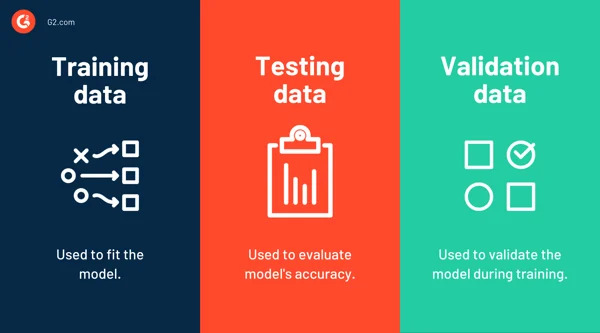
\includegraphics[width=7.5cm,height=4cm]{Pictures/ml-data/ml-datasets-type.jpg}
            \caption{Datasets: Types}
        \end{figure}
    \end{minipage}
    \hfill
    \begin{minipage}{0.45\textwidth}
        \begin{figure}[H]
            \centering
            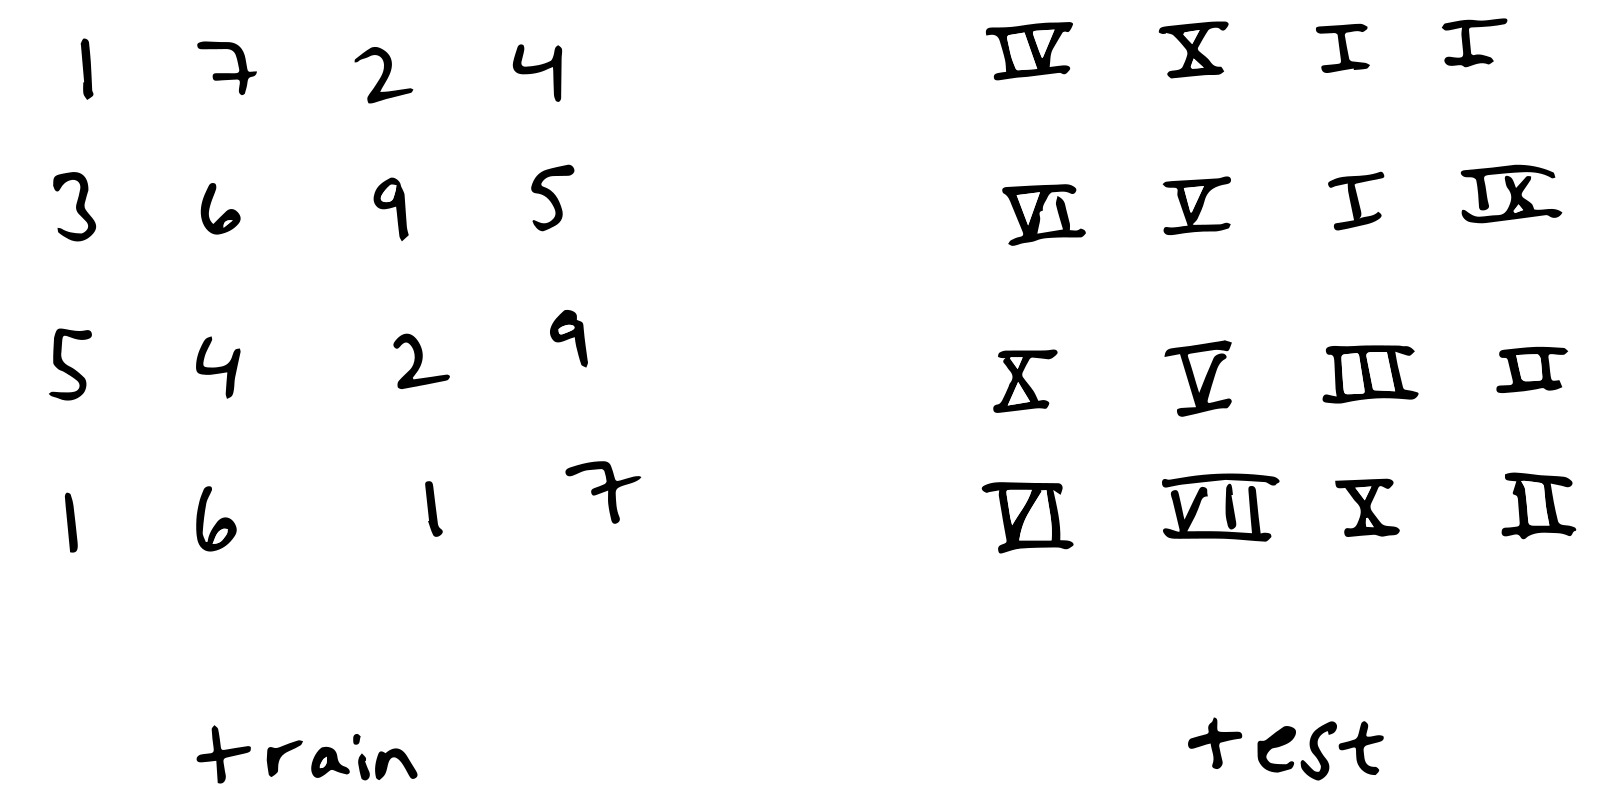
\includegraphics[width=7.5cm,height=4cm]{Pictures/ml-data/ml-data-distribution-shift.jpg}
            \caption{Distribution Shift}
        \end{figure}
    \end{minipage}
\end{table}




\subsection{Covariate shift / data shift \cite{dnn-1,mit-imbalance-outliers-shift}} \label{Covariate shift / data shift}
\begin{enumerate}
    \item Covariate shift occurs when $p(x)$ changes between train and test, but $p(y|x)$ does not. In other words, the distribution of inputs changes between train and test, but the relationship between inputs and outputs does not change.

    \item we assume that while the distribution of inputs may change over time, the labeling function, i.e., the conditional distribution $P(y | x)$ does not change. Statisticians call this covariate shift because the problem arises due to a shift in the distribution of the covariates (features).

    
\end{enumerate}

\vspace{0.2cm}
\textbf{Examples of covariate shift:}
\begin{enumerate}
    \item Self-driving car trained on the sunny streets of San Francisco and deployed in the snowy streets of Boston
    \item Speech recognition model trained on native English speakers and then deployed for all English speakers
    \item Diabetes prediction model trained on hospital data from Boston and deployed in India
\end{enumerate}

\subsubsection{Covariate Shift Correction \cite{dnn-1}} \label{Covariate Shift Correction}

\begin{customTableWrapper}{1.2}
\begin{table}[H]
    \centering
    \begin{tabular}{l l}
        $\dCurlyBrac{(\mathbf{x}_1, y_1), \ldots, (\mathbf{x}_n, y_n)}$ & training set \\

        $\dCurlyBrac{\mathbf{u}_1, \ldots, \mathbf{u}_m}$ & unlabeled test set \\

    \end{tabular}
\end{table}
\end{customTableWrapper}

\begin{enumerate}[itemsep=0.2cm]
    \item  For covariate shift, we assume that $\mathbf{x}_i$ for all $1 \leq i \leq n$ are drawn from some \textbf{source distribution} and $\mathbf{u}_i$ for all $1 \leq i \leq m$ are drawn from the \textbf{target distribution}.

    \item Assume that we want to estimate some dependency $P(y | x)$ for which we have labeled data $(\mathbf{x}_i, y_i)$.

    \item Unfortunately, the observations $x_i$ are drawn from some \textbf{source distribution} $q(x)$ rather than the \textbf{target distribution} $p(x)$.

    \item the dependency assumption means that the \textbf{conditional distribution does not change}: $p(y | x) = q(y | x)$.

    \item If the \textbf{source distribution} $q(x)$ is “\textbf{wrong}”, we can correct for that by using the following simple identity in the \textbf{risk} (SEE: \fullref{Empirical Risk and Risk}):
    \[
        \hfill
        \iint l(f(\mathbf{x}), y) p(y \mid \mathbf{x})p(\mathbf{x}) \;d\mathbf{x}dy =
        \iint l(f(\mathbf{x}), y) q(y \mid \mathbf{x})q(\mathbf{x})\dfrac{p(\mathbf{x})}{q(\mathbf{x})} \;d\mathbf{x}dy
        \hfill
    \]

    \item In other words, we need to reweigh each data example by the ratio of the probability that it would have been drawn from the correct distribution to that from the wrong one:
    $
        \beta_i \stackrel{\textrm{def}}{=} \dfrac{p(\mathbf{x}_i)}{q(\mathbf{x}_i)}
    $

    \item Plugging in the weight $\beta_i$ for each data example $(x_i, y_i)$ we can train our model using weighted empirical risk minimization:
    \[
        \hfill
        \displaystyle\mathop{\mathrm{minimize}}_f \dfrac{1}{n} 
        \dsum_{i=1}^n \beta_i l(f(\mathbf{x}_i), y_i)
        \hfill
    \]

    \item Alas, we do \textbf{NOT} know that ratio, so before we can do anything useful we need to estimate it.\\
    Many methods are available, including some fancy operator - theoretic approaches that attempt to recalibrate the expectation operator directly using a minimum-norm or a maximum entropy principle.\\
    Note that for any such approach, we need samples drawn from both distributions - the “true” $p$, e.g., by access to test data, and the one used for generating the training set $q$ the latter is trivially available).\\
    Note however, that we only need features $x \sim p(x)$; we do \textbf{NOT} need to access labels $y \sim p(y)$.

    \item For simplicity’s sake \textbf{assume} that we have an equal number of instances from both distributions $p(x)$ and $q(x)$, respectively.\\
    Now denote by $z$ labels that are $1$ for data drawn from $p$ and $-1$ for data drawn from $q$. Then the probability in a mixed dataset is given by:
    \[
        \hfill
        P(z=1 \mid \mathbf{x}) = \dfrac{p(\mathbf{x})}{p(\mathbf{x})+q(\mathbf{x})}
        \hfill
        \Rightarrow
        \dfrac{P(z=1 \mid \mathbf{x})}{P(z=-1 \mid \mathbf{x})} = \dfrac{p(\mathbf{x})}{q(\mathbf{x})}
        \hfill
    \]

    \item if we use a \textbf{logistic regression approach}, where $P(z=1 \mid \mathbf{x})=\dfrac{1}{1+\exp(-h(\mathbf{x}))}$ ($h$ is a parameterized function), it follows that:
    \[
        \hfill
        \beta_i = \dfrac{1/(1 + \exp(-h(\mathbf{x}_i)))}{\exp(-h(\mathbf{x}_i))/(1 + \exp(-h(\mathbf{x}_i)))} = \exp(h(\mathbf{x}_i))
        \hfill
    \]

    \item we need to solve two problems:
    \begin{enumerate}
        \item distinguish between data drawn from both distributions
        \item a weighted empirical risk minimization problem where we weigh terms by $\beta_i$
    \end{enumerate}

    \item prototypical algorithm for correcting covariate shift:
    \begin{enumerate}[itemsep=0.1cm]
        \item Create a binary-classification training set: $\{(\mathbf{x}_1, -1), \ldots, (\mathbf{x}_n, -1), (\mathbf{u}_1, 1), \ldots, (\mathbf{u}_m, 1)\}$

        \item Train a binary classifier using logistic regression to get the function $h$.

        \item Weigh training data using $\beta_i = \exp(h(\mathbf{x}_i))$ or better $\beta_i = \min(\exp(h(\mathbf{x}_i)), c)$ for some constant $c$.

        \item Use weights $\beta_i$ for training on $\{(\mathbf{x}_1, y_1), \ldots, (\mathbf{x}_n, y_n)\}$.

    \end{enumerate}

\end{enumerate}



\begin{table}[H]
    \begin{minipage}{0.45\textwidth}
        \begin{figure}[H]
            \centering
            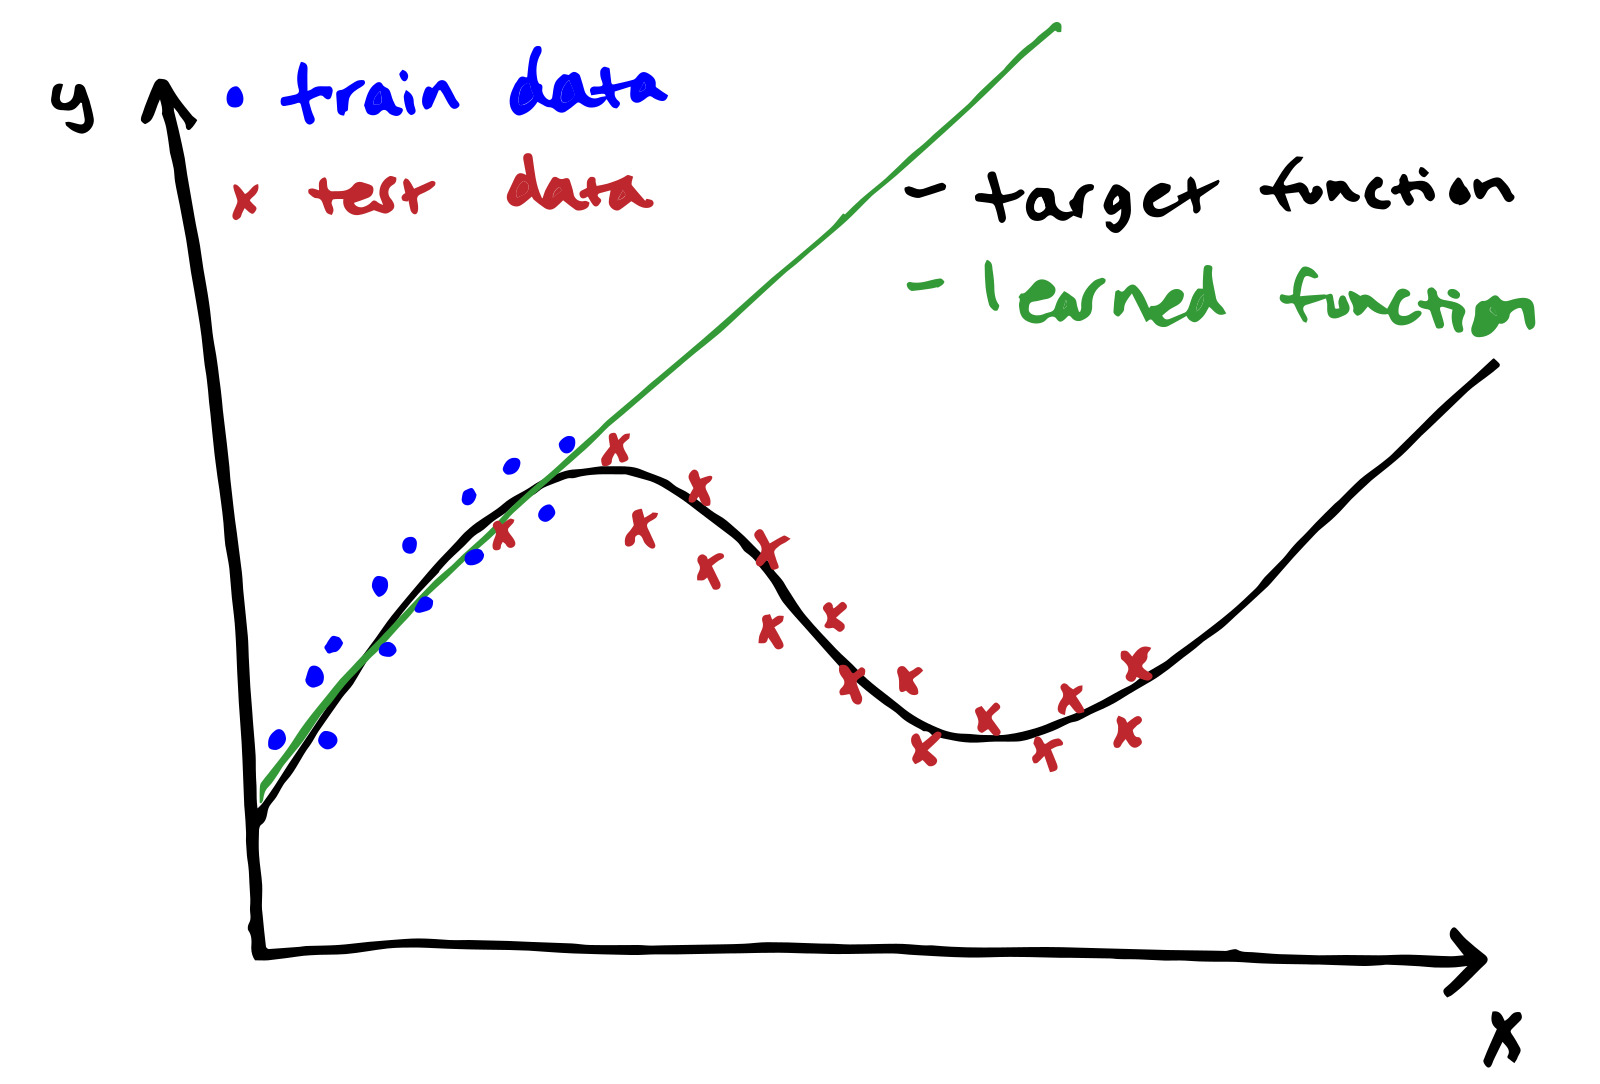
\includegraphics[width=7.5cm,height=4cm]{Pictures/ml-data/ml-data-covariate-shift.jpg}
            \caption{Distribution Shift: Covariate Shift/ Data Shift}
        \end{figure}
    \end{minipage}
    \hfill
    \begin{minipage}{0.45\textwidth}
        \begin{figure}[H]
            \centering
            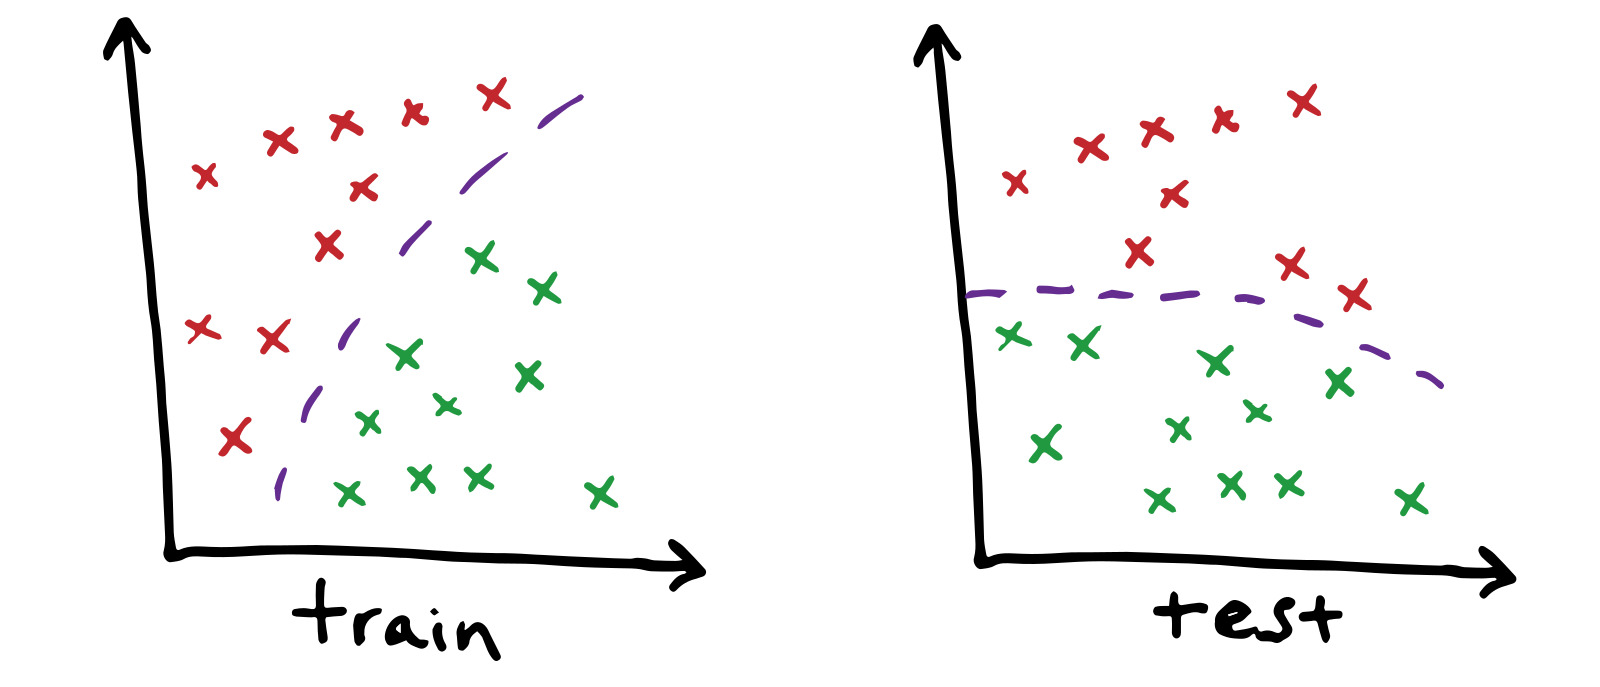
\includegraphics[width=7.5cm,height=4cm]{Pictures/ml-data/ml-data-concept-shift.jpg}
            \caption{Distribution Shift: Concept Shift}
        \end{figure}
    \end{minipage}
\end{table}




\subsection{Prior probability shift / label shift \cite{dnn-1,mit-imbalance-outliers-shift}} \label{Prior probability shift / label shift}
\begin{enumerate}
    \item Prior probability shift appears only in $y \to x$ problems (when we believe $y$ causes $x$). It occurs when label marginal $p(y)$ changes between train and test, but class-conditional distribution $p(x|y)$ remains fixed across domains. 
    
    \item You can think of it as the converse of covariate shift.
\end{enumerate}


\vspace{0.2cm}
\textbf{Examples:}
\begin{enumerate}
    \item If the model is trained on a balanced dataset of 50\% spam and 50\% non-spam emails, and then it’s deployed in a real-world setting where 90\% of emails are spam, that is an example of prior probability shift.

    \item we may want to predict diagnoses given their symptoms (or other manifestations), even as the relative prevalence of diagnoses are changing over time. Label shift is the appropriate assumption here because diseases cause symptoms.
\end{enumerate}

\subsubsection{Label Shift Correction \cite{dnn-1}} \label{Label Shift Correction}

\begin{customTableWrapper}{1.2}
\begin{table}[H]
    \centering
    \begin{tabular}{l l}
        $\mathbf{C}$ & confusion matrix ($k \times k$) \\
    \end{tabular}
\end{table}
\end{customTableWrapper}

\begin{enumerate}[itemsep=0.2cm]
    \item Assume that we are dealing with a classification task with $k$ categories.

    \item $q$ and $p$ are the \textbf{source distribution} (e.g., training time) and \textbf{target distribution} (e.g., test time), respectively.

    \item Assume that the distribution of labels shifts over time: $q(y) \neq p(y)$, but the \textbf{class-conditional distribution} stays the same: $q(x | y) = p(x | y)$.

    \item If the source distribution q(y) is “wrong”, we can correct for that according to the following identity in the risk:
    \[
        \hfill
        \iint l(f(\mathbf{x}), y) p(\mathbf{x} \mid y)p(y) \;d\mathbf{x}dy =
        \iint l(f(\mathbf{x}), y) q(\mathbf{x} \mid y)q(y)\dfrac{p(y)}{q(y)} \;d\mathbf{x}dy
        \hfill
    \]

    \item our importance weights will correspond to the label likelihood ratios: $\beta_i \stackrel{\textrm{def}}{=} \dfrac{p(y_i)}{q(y_i)}$

    \item One nice thing about label shift is that if we have a reasonably good model on the source distribution, then we can get consistent estimates of these weights without ever having to deal with the ambient dimension.

    \item To estimate the target label distribution, we first take our reasonably good off-the-shelf classifier (typically trained on the training data) and compute its “confusion” matrix using the validation set (also from the training distribution).

    \item In confusion matrix, where each column corresponds to the label category (ground truth) and each row corresponds to our model’s predicted category. Each cell’s value $c_{ij}$ is the fraction of total predictions on the validation set where the true label was $j$ and our model predicted $i$.

    \item we cannot calculate the confusion matrix on the target data directly because we do not get to see the labels for the examples that we see in the wild, unless we invest in a complex real-time annotation pipeline. What we can do, however, is average all of our model’s predictions at test time together, yielding the mean model outputs $\mu(\hat{\mathbf{y}}) \in \mathbb{R}^k$, where the $i^\textrm{th}$ element $\mu(\hat{y}_i)$ is the fraction of the total predictions on the test set where our model predicted $i$.

    \item under some mild conditions—if our classifier was reasonably accurate in the first place, and if the target data contains only categories that we have seen before, and if the label shift assumption holds in the first place (the strongest assumption here)—we can estimate the test set label distribution by solving a simple linear system
    \[
        \hfill
        \mathbf{C} p(\mathbf{y}) = \mu(\hat{\mathbf{y}})
        \hfill
    \]
    because as an estimate $\dsum_{j=1}^k c_{ij} p(y_j) = \mu(\hat{y}_i)$ holds for all $1 \leq i \leq k$, where $p(y_j)$ is the $j^\textrm{th}$ element of the k-dimensional label distribution vector p(y). If our classifier is sufficiently accurate to begin with, then the confusion matrix C will be invertible, and we get a solution $p(\mathbf{y}) = \mathbf{C}^{-1} \mu(\hat{\mathbf{y}})$.

    \item Because we observe the labels on the source data, it is easy to estimate the distribution $q(y)$. Then for any training example $i$ with label $y_i$, we can take the ratio of our estimated $p(y_i)/q(y_i)$ to calculate the weight $\beta_i$.
\end{enumerate}




\subsection{Concept shift \cite{dnn-1,mit-imbalance-outliers-shift}} \label{Concept shift}
\begin{enumerate}
    \item Concept shift occurs when $p(y|x)$ changes between train and test, but $p(x)$ does not. In other words, the input distribution does not change, but the relationship between inputs and outputs does. This can be one of the most difficult types of distribution shift to detect and correct.

    
\end{enumerate}


\vspace{0.2cm}
\textbf{Examples:}
\begin{enumerate}
    \item Predicting a stock price based on company fundamentals, trained on data from 1975 and deployed in 2023.
    
    \item Making purchase recommendations based on web browsing behavior, trained on pre-pandemic data and deployed in March 2020.
    
    \item We build a face detector. It works well on all benchmarks. Unfortunately it fails on test data—the offending examples are close-ups where the face fills the entire image (no such data was in the training set).

    \item We build a web search engine for the US market and want to deploy it in the UK.

    \item We train an image classifier by compiling a large dataset where each among a large set of classes is equally represented in the dataset, say 1000 categories, represented by 1000 images each. Then we deploy the system in the real world, where the actual label distribution of photographs is decidedly non-uniform.
\end{enumerate}


\subsubsection{Concept Shift Correction \cite{dnn-1}} \label{Concept Shift Correction}

\begin{enumerate}
    \item Concept shift is much harder to fix in a principled manner. 
    
    \item For instance, in a situation where suddenly the problem changes from distinguishing cats from dogs to one of distinguishing white from black animals, it will be unreasonable to assume that we can do much better than just collecting new labels and training from scratch. 
    
    \item Fortunately, in practice, such extreme shifts are rare.

    \item In such cases, we can use the same approach that we used for training networks to make them adapt to the change in the data.\\
    In other words, we use the existing network weights and simply perform a few update steps with the new data rather than training from scratch.
\end{enumerate}



\subsection*{SEE}
\begin{enumerate}
    \item \fullref{Covariate Shift (Data Shift) VS Concept Shift VS Prior Probability Shift (Label Shift)}

    \item \fullref{story: Model, environment and distribution shift}
    \item \fullref{Story: Covariate shift: Medical Diagnostics}
    \item \fullref{story: Distribution Shift: Self-Driving Cars}
    \item \fullref{story: Distribution Shift: Nonstationary Distributions}
\end{enumerate}


















